\Chapter{Mintaalkalmazás}

\Section{A mintaalkamazás célja}

% TODO: Le kellene írni, hogy a mintaalkalmazás arra szolgál, hogy ezzel lehet majd a bemutatásra kerülő keretrendszereket szépen összehasonlítani.

% TODO: Egy-két mondatban részletezni kellene, hogy az MMA micsoda, és hogy miért erre esett a választás.

\Section{Az alkalmazás specifikációja}

% TODO: Át kellene fogalmazni, mert itt nem a harcosokon kell a CRUD műveleteket végrehajtani.

A mintaalkalmazás egy MMA harcosokkal foglalkozó weboldal, ami megvalósítja a RESTful API-t, képes CRUD műveleteket végrehajtani a harcosokon, mint létrehozás, beolvasás, frissítés és törlés. A harcosok listáját egy kereső mezővel lehet szűrni, így változik az oldalon megjelenített lista a beírt szó hatására. Amennyiben a harcos neve tartalmazza a beírt betűsorozatot, akkor benne marad a listában, ha nem, akkor kikerül belőle.

Új harcost az "Add new fighter" feliratú gombbal lehet hozzáadni. Egy harcosnak a következő adatait lehet megadni:

\begin{itemize}
\item \textit{név}: egy szöveg mező, a harcos teljes neve, melynek minimum három karakter hosszúságúnak kell lennie, megadása kötelező,
\item \textit{becenév}: szintén szöveg mező, a harcos beceneve, nem kötelező megadni,
\item \textit{súlycsoport}: az előre megadott súlycsoportok közül a harcos súlycsoportjának kiválasztása, megadása kötelező, a választási lehetőségek száma: 3,
\item \textit{születési dátum}: dátum mező, a harcos születési ideje: év, hónap, nap formátumban, megadása kötelező,
\item \textit{szülőváros}: szöveg mező, a harcos szülőváros, megadása opcionális,
\item \textit{nemzetiség}: szöveg mező, a harcos nemzetisége, minimum két karakter, megadása kötelező,
\item \textit{magasság}: szám mező, a harcos magassága centiméterben megadva, 155 és 205 közé kell esnie, megadása kötelező,
\item \textit{súly}: szám mező, a harcos súlya kilogrammban értve, 50 és 120 közé kell, hogy essen, megadása kötelező,
\item \textit{record}: a harcos rekordja győzelem-döntetlen-vereség formában, megadása kötelező,
\item \textit{harcos avatárjának URL linkje}: szöveg mező, megadása kötelező,
\item \textit{a harcossal foglalkozó oldal URL linkje}: szöveg mező, megadása opcionális.
\end{itemize}

A harcosok főbb adatai, mint név, nemzetiség, születési dátum és rekord, a főoldalon (home) lévő "VIEW THE FIGHTERS" gombra kattintva jelennek meg. Minden harcos sorában egy "View Details" nevű gomb van, ami átirányít a "/fighter/details/:id" oldalra. Itt megtekinthetők az adott harcos további adatai, melyek fentebb kerültek felsorolásra. Továbbá ezen az oldalon tudjuk frissíteni az adatokat az "Edit" gombra kattintva.

Törölni a "Delete" nevű gombbal lehet. A "Go Back" gombbal a harcosokat megjelenítő oldalra tudunk visszanavigálni. A kitöltendő űrlap (form) az "Create" (létrehozás) esetén validációval van ellátva. A fent említett táblázatban szerepelnek a kitöltendő mezők leírásai, illetve a megadásukra vonatkozó megszorítások. A backend szolgáltatást a MongoDB adatbázis, a Node.js, mint szerver és a legnépszerűbb Node.js keretrendszer, az Express biztosítja, ami a HTTP kérések irányításáért felel.

Frontend részről, mint személyes preferált keretrendszer az AngularJS és Angular 2, ezeken kívül a React.js, és a Vue.js került implementálásra.

Az alkalmazás elindítása után a "Login" gombra kattintva felugrik az Auth0 szervíz bejelentkező és regisztrációs képernyője, ahol a felhasználó létrehozhat egy új fiókot, vagy bejelentkezhet a Facebook vagy a Google szolgáltatással, ezt követően a program átirányítja a főoldalra. (\ref{fig:home}. ábra).

\begin{figure}[htb]
\centering
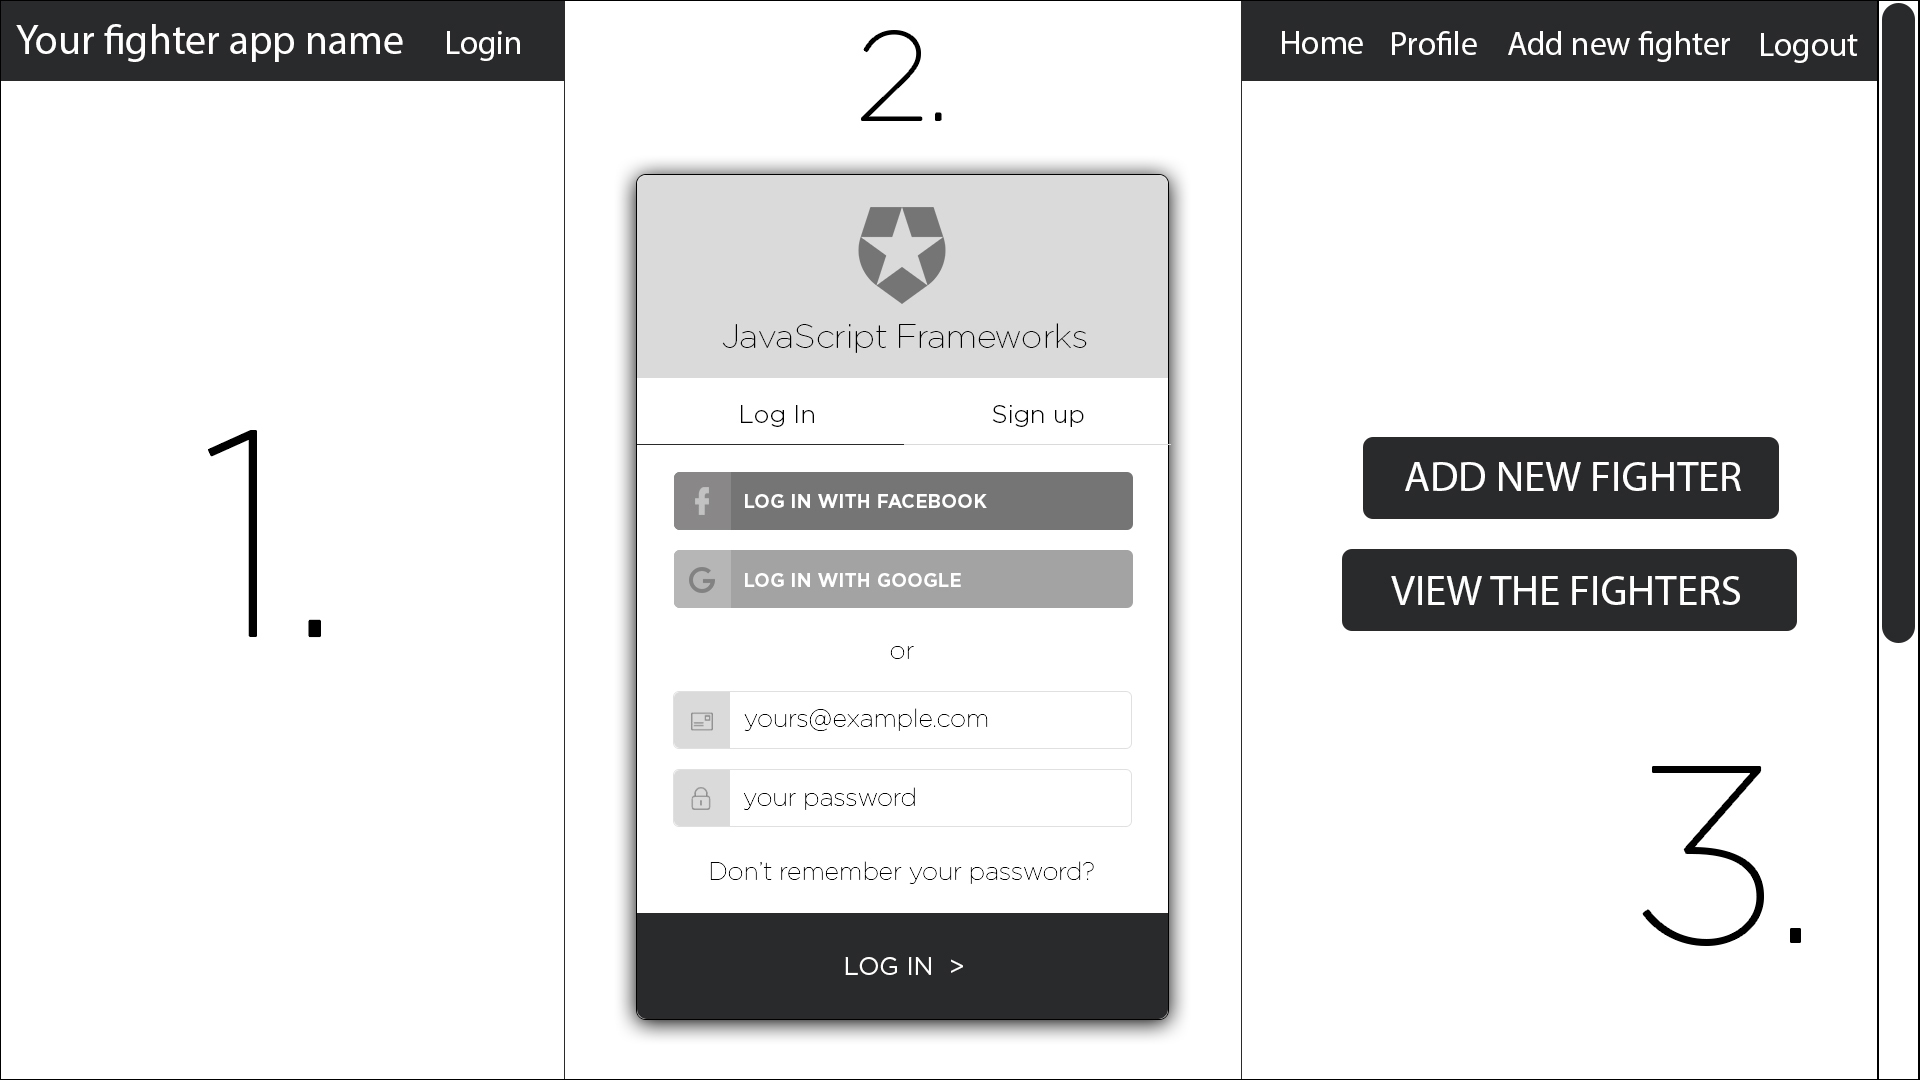
\includegraphics[scale=0.7]{kepek/login_auth0_home.jpg}
\caption{Főoldal (Home)}
\label{fig:home}
\end{figure}

A "VIEW THE FIGHTERS" feliratú linkre kattintva a "/fighters" oldal jelenítődik meg a harcosok listájával (\ref{fig:search_bar}. ábra).

\begin{figure}[htb]
\centering
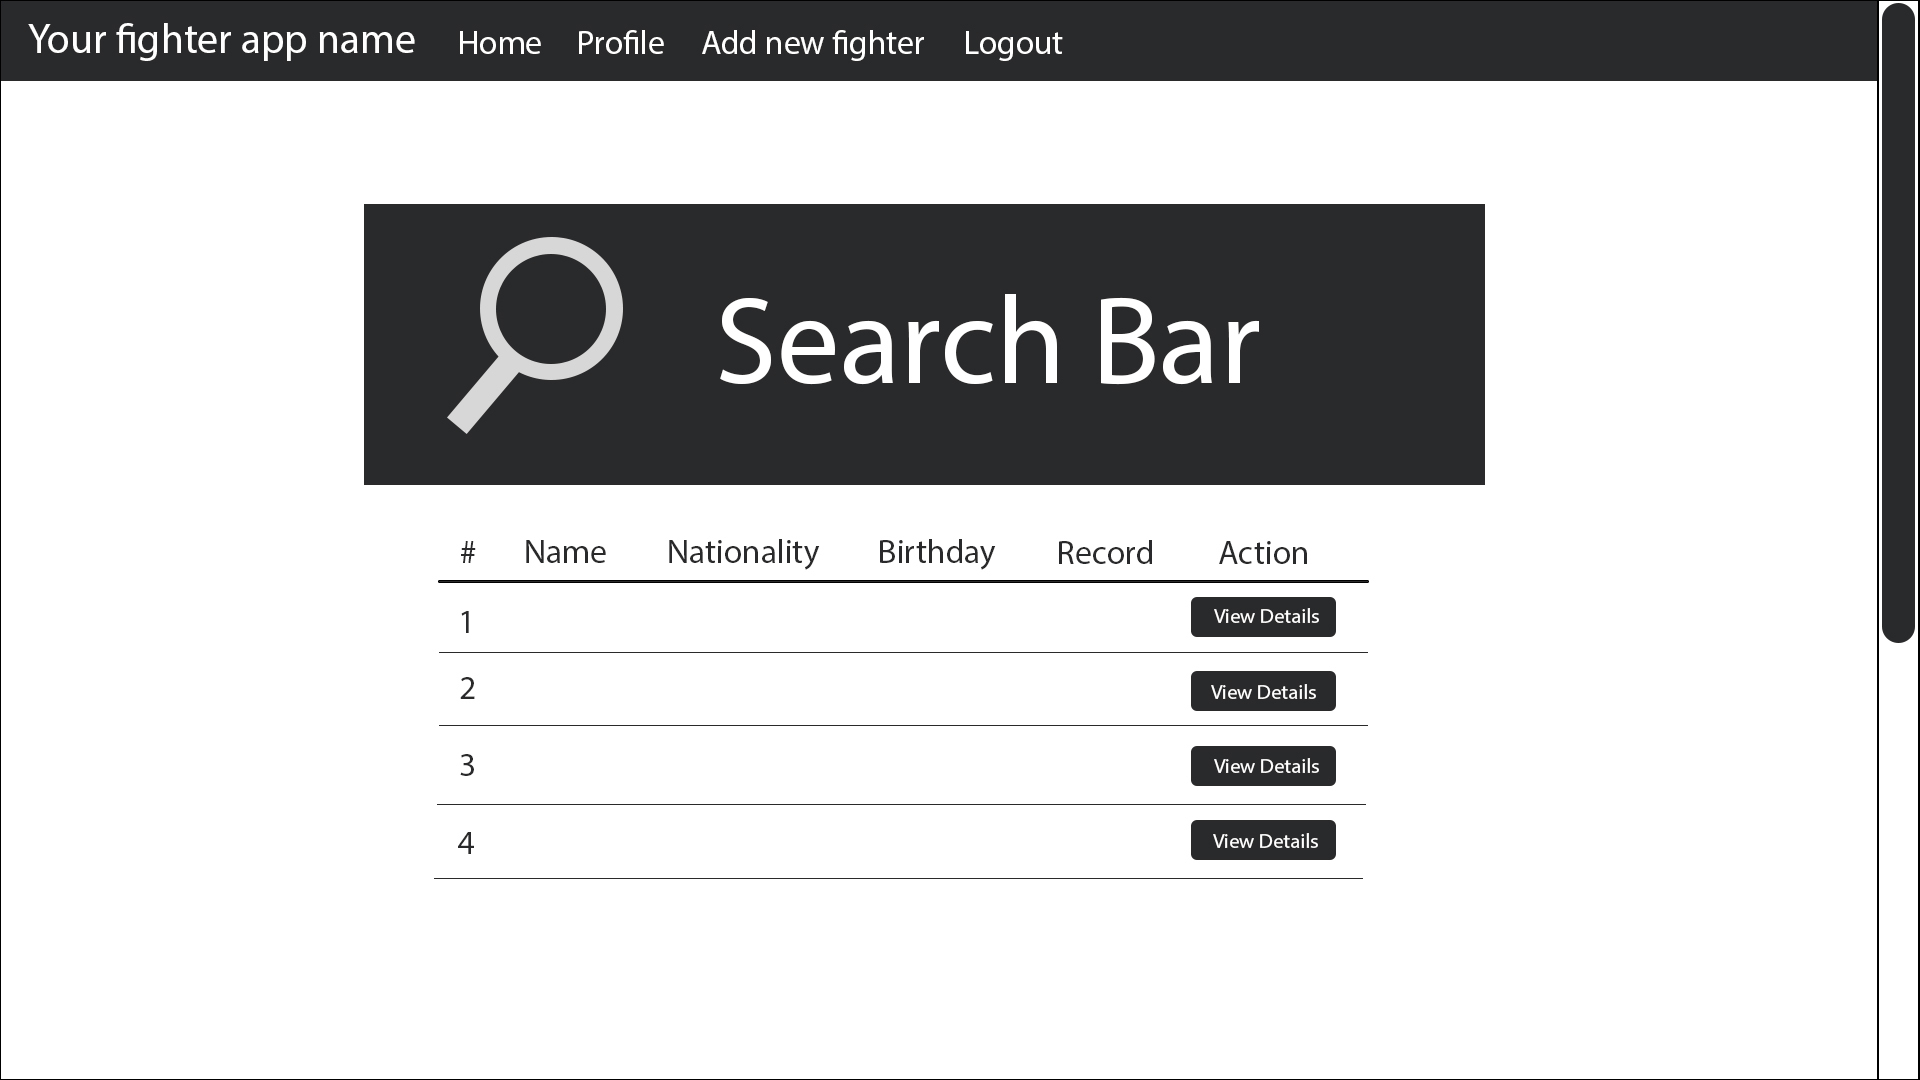
\includegraphics[scale=0.7]{kepek/search_bar.jpg}
\caption{Harcos lista oldal (\textit{Fighters})}
\label{fig:search_bar}
\end{figure}

\begin{figure}[htb]
\centering
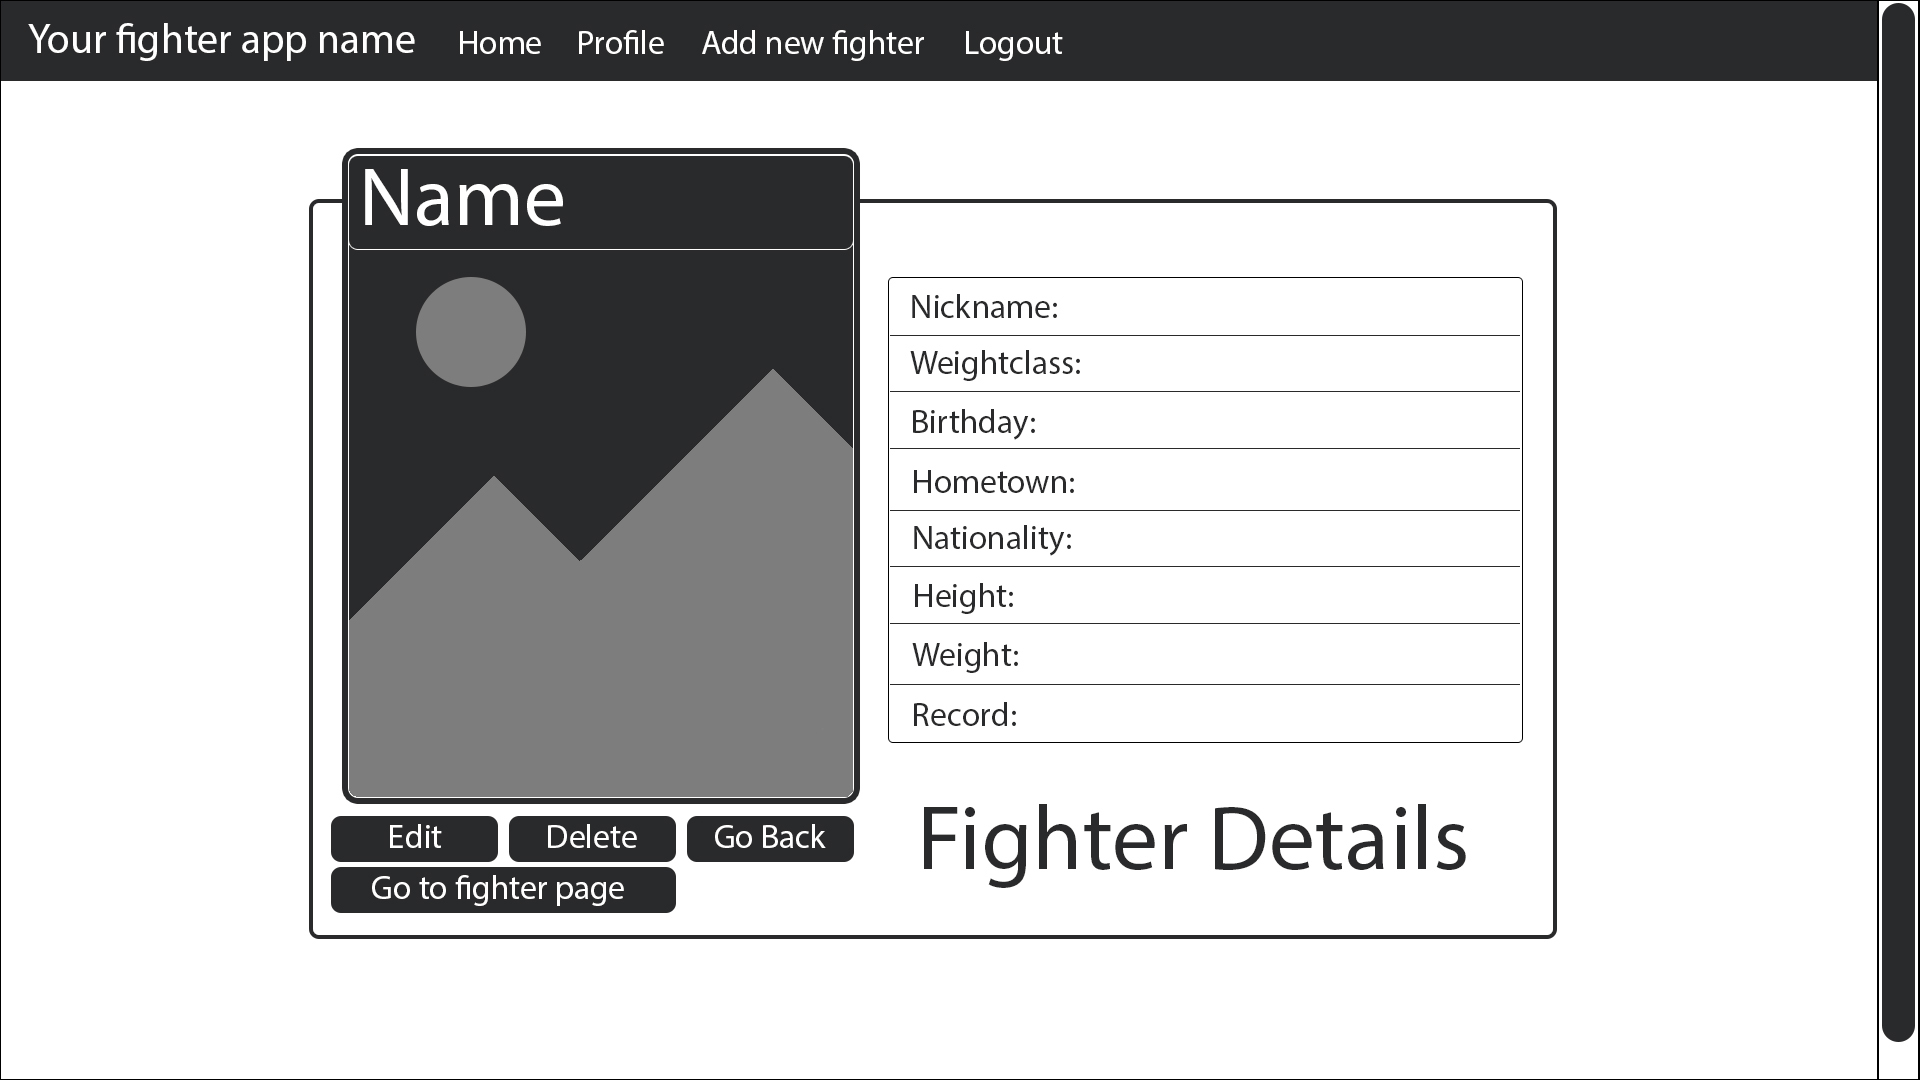
\includegraphics[scale=0.7]{kepek/details.jpg}
\caption{Harcos adatait megjelenítő oldal (\textit{Fighter Details})}
\label{fig:details}
\end{figure}

A harcos sorában lévő "View Details" linkre kattintva az adott harcos adatait tartalmazó oldal jelenik meg az "/fighters/details/id" oldalon (\ref{fig:details}. ábra).

Ezen az oldalon az "Edit" gombra kattintva a program átirányítja a felhasználót a "/fighters/edit/:id" oldalra, ahol a harcos adatait tudja frissíteni (\ref{fig:edit}. ábra).

\begin{figure}[htb]
\centering
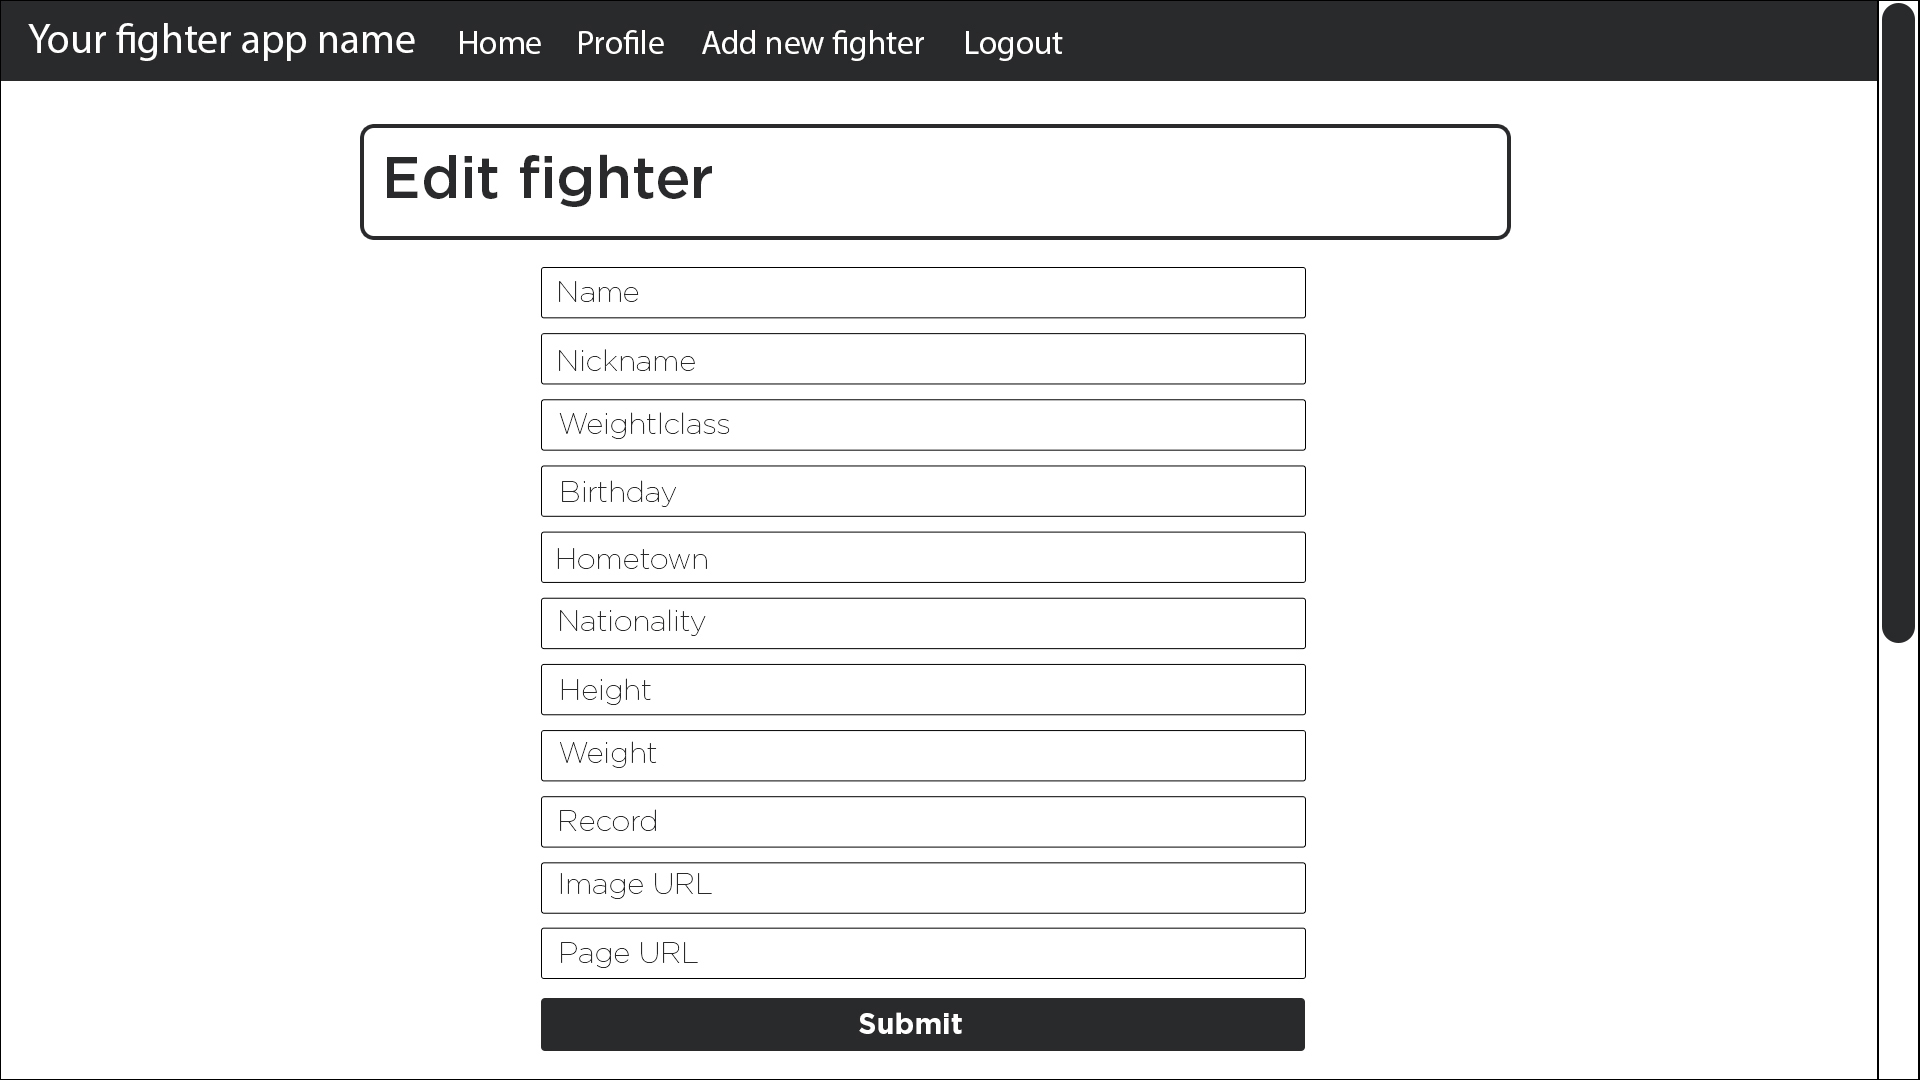
\includegraphics[scale=0.7]{kepek/edit_fighter.jpg}
\caption{Oldal a harcosok adatainak szerkesztéséhez (\textit{Edit Fighter Details})}
\label{fig:edit}
\end{figure}

\begin{figure}[htb]
\centering
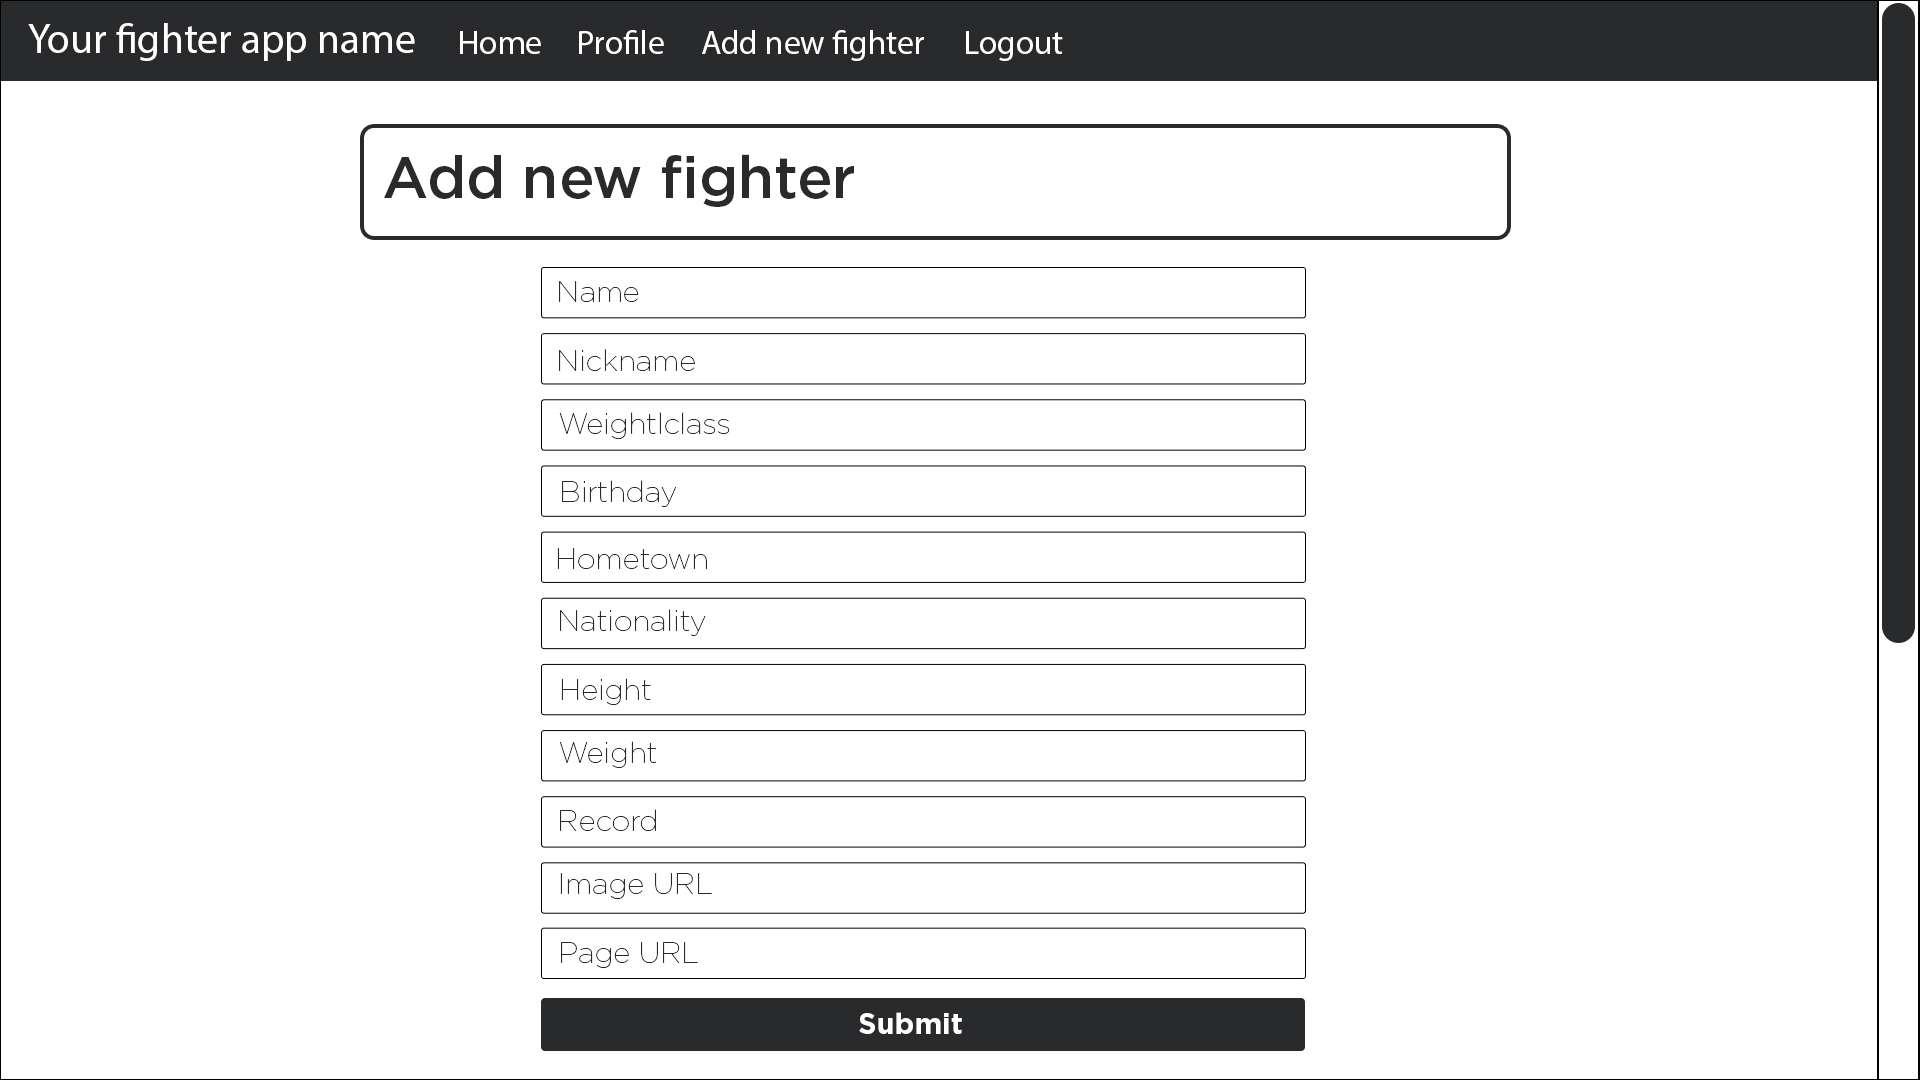
\includegraphics[scale=0.7]{kepek/add_new_fighter.jpg}
\caption{Új harcost létrehozó oldal (\textit{Add new fighter})}
\label{fig:add}
\end{figure}
\newpage
Végül, ha a felhasználó bejelentkezés után (\ref{fig:home}. ábra), az "ADD NEW FIGHTER" feliratú gombra kattint, akkor a "/fighters/add" oldal ugrik fel (\ref{fig:add}. ábra).
